\documentclass[11pt]{article}
\usepackage{fullpage,amsmath,amsfonts,mathpazo,microtype,nicefrac,graphicx}

% Set-up for hypertext references
\usepackage{hyperref,color,textcomp}
\definecolor{webgreen}{rgb}{0,.35,0}
\definecolor{webbrown}{rgb}{.6,0,0}
\definecolor{RoyalBlue}{rgb}{0,0,0.9}
\hypersetup{
   colorlinks=true, linktocpage=true, pdfstartpage=3, pdfstartview=FitV,
   breaklinks=true, pdfpagemode=UseNone, pageanchor=true, pdfpagemode=UseOutlines,
   plainpages=false, bookmarksnumbered, bookmarksopen=true, bookmarksopenlevel=1,
   hypertexnames=true, pdfhighlight=/O,
   urlcolor=webbrown, linkcolor=RoyalBlue, citecolor=webgreen,
   pdfauthor={Chris H. Rycroft},
   pdfsubject={Harvard AM205 (Fall 2014)},
   pdfkeywords={},
   pdfcreator={pdfLaTeX},
   pdfproducer={LaTeX with hyperref}
}
\hypersetup{pdftitle={AM205: Assignment 2}}

% Macro definitions
\newcommand{\N}{\mathbb{N}}
\newcommand{\Z}{\mathbb{Z}}
\newcommand{\Q}{\mathbb{Q}}
\newcommand{\R}{\mathbb{R}}
\newcommand{\B}{\mathbb{B}}
\newcommand{\p}{\partial}
\newcommand{\Trans}{\mathsf{T}}
\renewcommand{\vec}[1]{\mathbf{#1}}
\newcommand{\vx}{\vec{x}}
\newcommand{\vb}{\vec{b}}

\DeclareMathOperator{\rank}{rank}

\begin{document}
\section*{AM205: Assignment 2 (due 5~PM, October 10)}
\noindent{\it Program files: A number of program and data files for this
homework can be downloaded as a single ZIP file from the course website.}

\begin{enumerate}
  \item {\bf Norms and Newton root-finding.} Define a matrix
    \begin{equation}
      A=\left[
      \begin{array}{cc}
	3 & -1 \\
	1 & 0
      \end{array}
      \right],
    \end{equation}
    which represents a linear transformation in $\R^2$.
    \begin{enumerate}
      \item Find four points $b \in \R^2$ such that $||b||_2 = 1$ and
	$||Ab||_2=1$. Plot the two curves $||x||_2=1$ and $||Ax||_2=1$ and mark
	the points $b$ on this plot.
      \item Find four points $c \in \R^2$ such that $||c||_\infty = 1$ and
	$||Ac||_\infty=1$. Plot the two curves $||x||_\infty=1$ and
	$||Ax||_\infty=1$ and mark the points $c$ on this plot.
      \item Consider the function $f:\R^2 \to \R^2$ defined as 
	\begin{equation}
	  f(d)=( ||d||_4-1, ||Ad||_4-1),
	\end{equation}
	where $d\in \R^2$. Write a program to find four solutions to the
	equation $f(d)=(0,0)$ using the vector generalization of the Newton
	root finding method.\footnote{You can make use of linear algebra
	routines in your code, but the actual Newton iteration should be coded
	yourself, without using a library function.} Plot the two curves
	$||x||_4=1$ and $||Ax||_4=1$ and mark the solutions $d$ on this plot.
      \item Show that the families of points $b$, $c$, and $d$ (12 points in
	total) lie on two straight lines, and explain why this is true.
    \end{enumerate}
  \item {\bf LU factorization for binary numbers.} In this course we usually
    calculate using the set of real numbers $\R$. This question takes
    a different approach of calculating using the binary set $\B=\{0,1\}$ with
    just two elements. Within $\B$, addition is defined as
    \[
    0+0=0, \qquad 0+1 = 1, \qquad 1+1=0,
    \]
    corresponding to regular addition, and then taking the remainder after
    division by two. Multiplication is defined as
    \[
    0\times0=0, \qquad 0\times 1 = 0, \qquad 1\times 1= 1.
    \]
    Subtraction is the same as addition, so that $x-y=x+y$ for all $x,y\in \B$.
    For division, $x/1=x$ for all $x\in \B$, and $x/0$ is undefined, giving a
    ``division by zero'' error. With these rules $\B$ becomes a {\it
    field},\footnote{More specifically, $\B$ is the
    \href{http://en.wikipedia.org/wiki/Modular_arithmetic}{field of integers
    modulo $p$} for $p=2$, which is frequently studied in number theory
    courses.} in that addition and muliplication have all the usual properties.
    In most cases, linear algebra calculations that work for numbers in $\R$
    will work just as well for numbers in $\B$, as long as the arithmetic
    operations are interpreted as defined above.

    There are various ways to write programs that calculate in $\B$. In the homework
    files, there are programs \texttt{bin\_\,mul.py} and \texttt{bin\_\,mul.m}
    that demonstrate this in Python and MATLAB, respectively. They both
    implement matrix multiplication in $\B$, using the test matrices
    \[
    L=\left[
    \begin{array}{cccc}
      1 & 0 & 0 & 0 \\
      0 & 1 & 0 & 0 \\
      1 & 1 & 1 & 0 \\
      1 & 0 & 1 & 1
    \end{array}
    \right],
    \quad
    U=\left[
    \begin{array}{cccc}
      1 & 0 & 1 & 0 \\
      0 & 1 & 1 & 1 \\
      0 & 0 & 1 & 0 \\
      0 & 0 & 0 & 1
    \end{array}
    \right],
    \quad
    A=\left[
    \begin{array}{cccc}
      1 & 0 & 1 & 0 \\
      0 & 1 & 1 & 1 \\
      1 & 1 & 1 & 1 \\
      1 & 0 & 0 & 1
    \end{array}
    \right].
    \]
    The two programs calculate $LU$ and show that it is equal to $A$. We now
    consider adapting the algorithms presented in class to carry out the LU
    factorization to solve linear systems in $\B$.
    \begin{enumerate}
      \item Write a function \texttt{fsolve} that takes a lower triangular
	matrix $L$ and vector $b$ and returns the solution $x$ to the linear
	system $Lx=b$ using forward substitution described in the lectures.
	If any diagonal element of $L$ is zero, the function should give
	an error and report that the matrix is singular.
      \item Write a function \texttt{rsolve} that takes an upper triangular
	matrix $U$ and vector $b$ and returns the solution $x$ the the linear
	system $Ux=b$ using reverse substitution described in the lectures.
	If any diagonal element of $U$ is zero, the function should give
	an error and report that the matrix is singular.
      \item Write a program to calculate the LU factorization with
	partial pivoting as described in the
	\href{http://iacs-courses.seas.harvard.edu/courses/am205/slides/am205_lec07.pdf}{lecture
	7 slides}. The program should return $P$, $L$, and $U$ so that
	$PA=LU$, and it should also work on singular matrices.
      \item In the homework files, there are two directories called
	\texttt{q2\_\,small} and \texttt{q2\_\,large}. Each has a text file
	containing a binary matrix $A$ and a text file containing source data
	$b$. Find the solutions $x$ to both linear systems $Ax=b$.
      \item {\bf Optional.} What is the probability that a
	random $n\times n$ binary matrix will be singular?
    \end{enumerate}
  \item {\bf The light game.} An electronic children's toy consists of a
    $7\times 7$ grid of lights, which are initially all switched off. Pressing
    on a light toggles it on or off, and toggles its orthogonally adjacent
    neighbors on or off. A single press in the interior of the grid therefore
    creates set of lights in the shape of a plus sign, while several presses
    may lead to more complicated patterns. Three examples of the lights after
    different presses $(i,j)$ are shown below.
    \setlength{\unitlength}{0.85bp}
    \begin{center}
      \begin{picture}(490,140)(0,0)
	\put(21,15){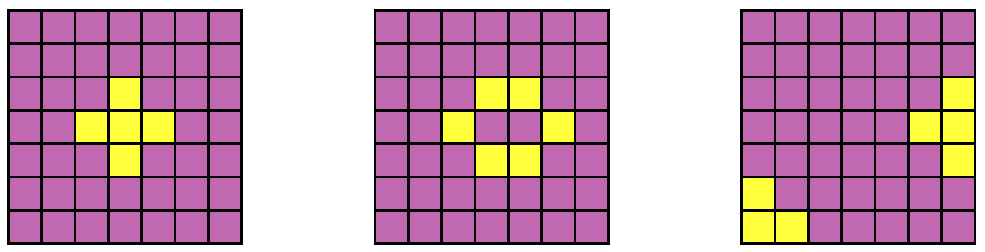
\includegraphics[scale=0.85]{lights1}}
	\small
	\put(82,3){\makebox(0,0)[c]{Press $(3,3)$}}
	\put(258,3){\makebox(0,0)[c]{Press $(3,3)$ and $(3,4)$}}
	\put(434,3){\makebox(0,0)[c]{Press $(6,0)$ and $(3,6)$}}
	\scriptsize
	\put(0,120){$i=0$}
	\put(0,24){$i=6$}
	\put(23,136){$j=0$}
	\put(119,136){$j=6$}
	\put(176,120){$i=0$}
	\put(176,24){$i=6$}
	\put(199,136){$j=0$}
	\put(295,136){$j=6$}
	\put(352,120){$i=0$}
	\put(352,24){$i=6$}
	\put(375,136){$j=0$}
	\put(471,136){$j=6$}
      \end{picture}
    \end{center}
    \begin{enumerate}
      \item Let $x$ be a vector in $\B^{49}$ that represents which lights
	have been pressed, and let $b$ be a vector in $\B^{49}$ that
	represents which lights are lit. Write a program that creates a
	$49\times 49$ binary matrix $A$ such that
	\begin{equation}
	  Ax=b
	  \label{eq:lights}
	\end{equation}
	in the binary arithmetic scheme introduced in Question 2.
      \item The toy presents different patterns of lights and the aim is to
	determine the correct presses to switch off all of the lights. For each
	of the patterns given below, use your binary LU solver from Question 2
	to determine the correct presses.
	\begin{center}
	  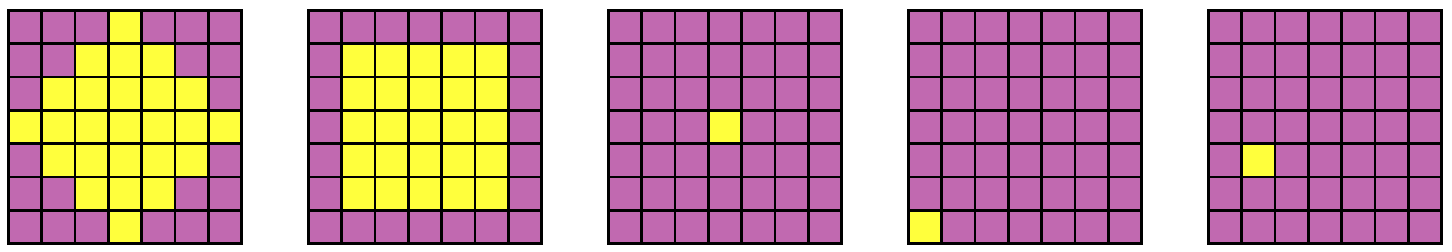
\includegraphics[scale=0.55]{lights2}
	\end{center}
	For each case, present your results as in a $7\times 7$ grid, such as
	by using the \texttt{spy} command in NumPy and MATLAB. In addition,
	create a light pattern of your own and solve it.
      \item For the $7\times 7$ grid the matrix $A$ in Eq.~\ref{eq:lights} is
	non-singular, so that every combination of lights can be created with
	presses. However, this is not always the case for a general $m\times n$
	grid. For each $m\times n$ grid with $m,n\in \{1,2,\ldots,9\}$
	determine the dimension of the
	\href{http://en.wikipedia.org/wiki/Kernel_(linear_algebra)}{null
	space}, $f(m,n)=mn-\rank A$.\footnote{Note that $f(m,n)$ is equal to
	the number of zero diagonal entries in $U$, in the LU factorization of $A$.}
      \item {\bf Optional.} For the $5\times 5$ grid, find four linearly
	independent press patterns that leave all of the lights switched off.
    \end{enumerate}
  \item {\bf Difficult cases for LU factorization.} Matrices of the form 
      \begin{equation}
	G_n =
	\left[
	\begin{array}{cccccc}
	 1 &0 &0 &0&\ldots &1\\
	 -1 &1 &0 &0&\ldots &1\\
	 -1 &-1 &1 &0&\ldots &1\\
	 -1 &-1 &-1 &1&\ldots &1\\
	 \vdots & & & & \ddots & \vdots\\
	-1 & -1 & -1 &-1& \ldots & 1
	\end{array}
	\right]
      \end{equation}
    in $\R^{n\times n}$ are examples of the very rare cases in which Gaussian elimination is unstable.
    \begin{enumerate}
      \item Write a function \texttt{generate\_\,g} that returns $G_n$.
      \item Write a program that measures the time $t(n)$ taken to run
	\texttt{generate\_\,g} as a function of $n$, for $n=10,20,\ldots,1000$.
	Make a plot of $t(n)$ as a function of $n$.\footnote{For examples of
	how to time functions, see the \texttt{lu\_\,time.py} and
	\texttt{chol\_\,time.py} examples from lecture 8.} You should find that
	the $t(n)\sim \alpha t^\beta$. Determine $\alpha$ and $\beta$ and
	discuss whether the value of $\beta$ is reasonable, given the number of
	operations that \texttt{generate\_\,g} does.
      \item For $n = 10, 20, \ldots, 200$, set $x = [1,1,\ldots,1]^T \in \R^n$ and
	construct a right-hand side vector $b= G_n x$. Solve the system
	$G_n \hat{x} = b$ using the LU factorization.\footnote{In NumPy
	the routine \texttt{numpy.linalg.solve} uses the LU factorization.
	In MATLAB, the ``backslash'' operator uses the LU factorization.}
	Plot the 2-norm relative error as a function of $n$ and explain why
	we consider Gaussian elimination with partial pivoting to be
	numerically unstable in this case. In addition, make a plot that
	shows that the inequality
	\begin{equation}
	  \frac{\|x - \hat x\|_2}{\|\hat x\|_2} \leq \kappa(G_n,2)\frac{\|r(\hat x)\|_2}{\|A\|_2\|\hat x\|_2}
	\end{equation}
	is satisfied, where $\kappa(G_n,2)$ is the condition number of $G_n$
	with respect to the 2-norm.
    \end{enumerate}
  \item {\bf Singular Value Decomposition (SVD) and Principal Component Analysis (PCA).} Suppose we are given a data set represented by a matrix $X \in \R^{m\times n}$. One way to analyze this data is to perform PCA, which consists of computing the eigenvalue decomposition of the matrix $XX^\Trans$. The eigenvectors of $XX^\Trans$ are referred to as principal components, and the eigenvalues related to the variance in the data set associated with the principal components.
    \begin{enumerate}
      \item We discussed the relationship between the eigenvalue decomposition
	of $XX^\Trans$ and the SVD of $X$ in lectures. Based on this
	relationship, show that the principal components are the same as the
	left singular vectors of $X$.
      \item It can be less accurate to perform PCA by computing eigenvalues of
	$XX^\Trans$ as opposed to using the SVD. For example, consider the
	matrix
	\begin{equation}
	  X =
	  \left[
	  \begin{array}{ccccc}
	    1 & 10^{-8} & 0 & 0 & 0 \\
	    1 & 0 & 10^{-8} & 0 & 0 \\
	    1 & 0 & 0 & 10^{-8} & 0 \\
	    1 & 0 & 0 & 0 & 10^{-8}
	  \end{array}
	  \right].
	\end{equation}
	What are the exact eigenvalues of $XX^\Trans$? You can either find
	these by hand, or you can make use of a symbolic computing environment
	like Mathematica or Maple.
      \item Write a program to numerically compute (i) the eigenvalues of
	$XX^\Trans$, and (ii) the squares of the singular values of $X$.
	Which method, (i) or (ii), is better in this case?
      \item We will now make use of PCA to analyze the data provided in the file \texttt{q5.txt}. Recall from linear algebra that the orthogonal projection of a vector $x \in \R^m$ onto a subspace $W$ of $\R^m$ is is defined as
	\begin{equation}
	  v^\Trans(Px-x) = 0 \qquad \forall v \in W,
	\end{equation}
	where $Px \in W$ denotes the projection of $x$ onto $W$. This formula
	states that the projection error $Px - x$ is orthogonal to $W$. The
	principal components of $X$ provide an orthogonal basis that we can use
	to form a low-dimensional approximation to $X$ via orthogonal
	projection. Compute the orthogonal projection of each column of $X$
	onto the first two principal components, and form a 2D scatter plot of
	the projected data. In your plot, the coefficients of the first and
	second principal components should correspond to the horizontal and
	vertical axes, respectively.
      \item The total projection error in part (c) is given by
	\begin{equation}
	  E_P = \left( \sum_{j=1}^{20} ||Px_j - x_j||_2^2 \right)^{1/2},
	  \label{eq:pcaproj}
	\end{equation}
	where $x_j$ denotes the $j$th column of $X$. Give an analytical formula
	for $E_P$ that involves the singular values of $X$. {\it (Hint: For $P$
	denoting the orthogonal projection operator onto the span of the first
	two principal components, it can be shown that the matrix $[Px_1 | Px_2
	| \dots | Px_n] \in \R^{10\times20}$ minimizes the total projection
	error, as defined in Eq.~\ref{eq:pcaproj}, among all rank 2 matrices.)}

	In addition, calculate $E_P$ directly based on your results for $P x_j$
	for $j = 1, \ldots , 20$ from (a). Verify that your calculated value
	agrees with the result of evaluating your analytical formula for $E_P$.
    \end{enumerate}
\end{enumerate}
\end{document}
